\section{About The Robot}
\subsection{Robot Structure}

The construction of our robot took about 1.5 weeks.
We managed to make the robot structure as compact as possible, so that it takes minimal space within the maze.
The dimensions of the robot can be seen in figure \ref{fig:robot_dim}.

%\begin{figure} 
%  \centering 
%  \subfigure[A]{ 
%    \label{fig:subfig:a} %% label for first subfigure 
%    \includegraphics[width=1.0in]{robot.jpg}} 
%  \hspace{1in} 
%  \subfigure[Big Box]{ 
%    \label{fig:subfig:b} %% label for second subfigure 
%    \includegraphics[width=1.5in]{dimentions.png}} 
%  \caption{Two Subfigures} 
%  \label{fig:subfig} %% label for entire figure 
%\end{figure}

\begin{figure}
\centering

\begin{subfigure}[t]{0.4\textwidth}
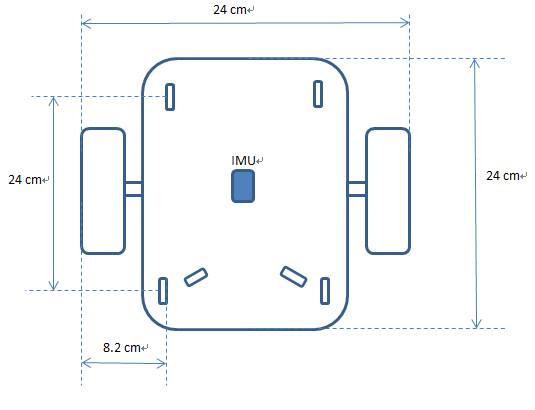
\includegraphics[width=\textwidth]{figures/dimensions.jpg}
\caption{Top View and Sensor Placements} 
\label{fig:robot_dim}
\end{subfigure}
%\hfill
\quad
\begin{subfigure}[t]{0.4\textwidth}
\includegraphics[width=\textwidth]{figures/robot.png}
\caption{Front} 
\label{fig:robot}
\end{subfigure}

\caption{Robot}
\end{figure}

\setlength{\parindent}{0pt}Since the robot is constructed with the same length and width of 24cm, when it turns, it will never hit the front wall as long as there was space left in front before it turns.
The robot has two layers. On the bottom layer, motors, wheels are mounted in the center and all sensors are fixed on this layer as well.
On the top layer, the Arduino board, the camera braket are fixed.
Also there are two holes in the top layer, where the NUC and the battery is placed.
Since the NUC is standing between two layers with its USB connectors facing sideways, the usb interfaces are hard to reach and are close to the wheels when plugged in.
A change in the overall construction was avoided by bending the cables tightly upwards.

\subsection{Sensor Placement}
There are 6 IR sensors and one IMU sensor integrated at the center of the lower plate.
On each side of the robot, two short range IR sensors are mounted with distance in-between as far as possible, in order to get a better estimation of the robot angle. 
And two long range IR sensors pointed to the front with an angle adjustment to the robot center.  
The reason why the front IR sensors are not pointed directly to the front is because if we do that, when there are obstacles come to the area exactly between the two front sensors, nothing will be detected.
With crossed sensors, an triangle area will be formed, thus it guarantees front obstacle detection.
Actually, we took advantages of such placement when dealing with the 'wall of death '.\\

\setlength{\parindent}{0pt}There is also an IMU sensor mounted on the bottom layer, we used it for detection of crash. When the robot crashes into an obstacle, the IMU will send the current time to brain to reset.
And the robot will try to go backwards and continue its path again.

\subsection{Camera Placement}
Since the PrimeSense has a minimal working range of 35 cm, the camera is fixed on top of an aluminum tower with height of 28cm above the floor. 
The system is not sensitive to the camera angle since software calibration of camera angle will be executed when the vision is started.
Thus we are able to give position of detected objects precisely without caring a lot about the camera angle.

